Hier zijn de resultaten van het project:
\subsection{Hardware}
\label{subsec:results:hardware}
Zie figuur \ref{fig:voorvoor} en \ref{fig:voorachter} van de vóór- en achterkant van de Tetris gameboy, van vóór de (meeste) bedradingen. Deze foto's bevatten maar paar van de bedradingen, omdat er geen foto's zijn gemaakt van dat er géén bedrading zijn. 
\begin{figure}[h]
    \centering
    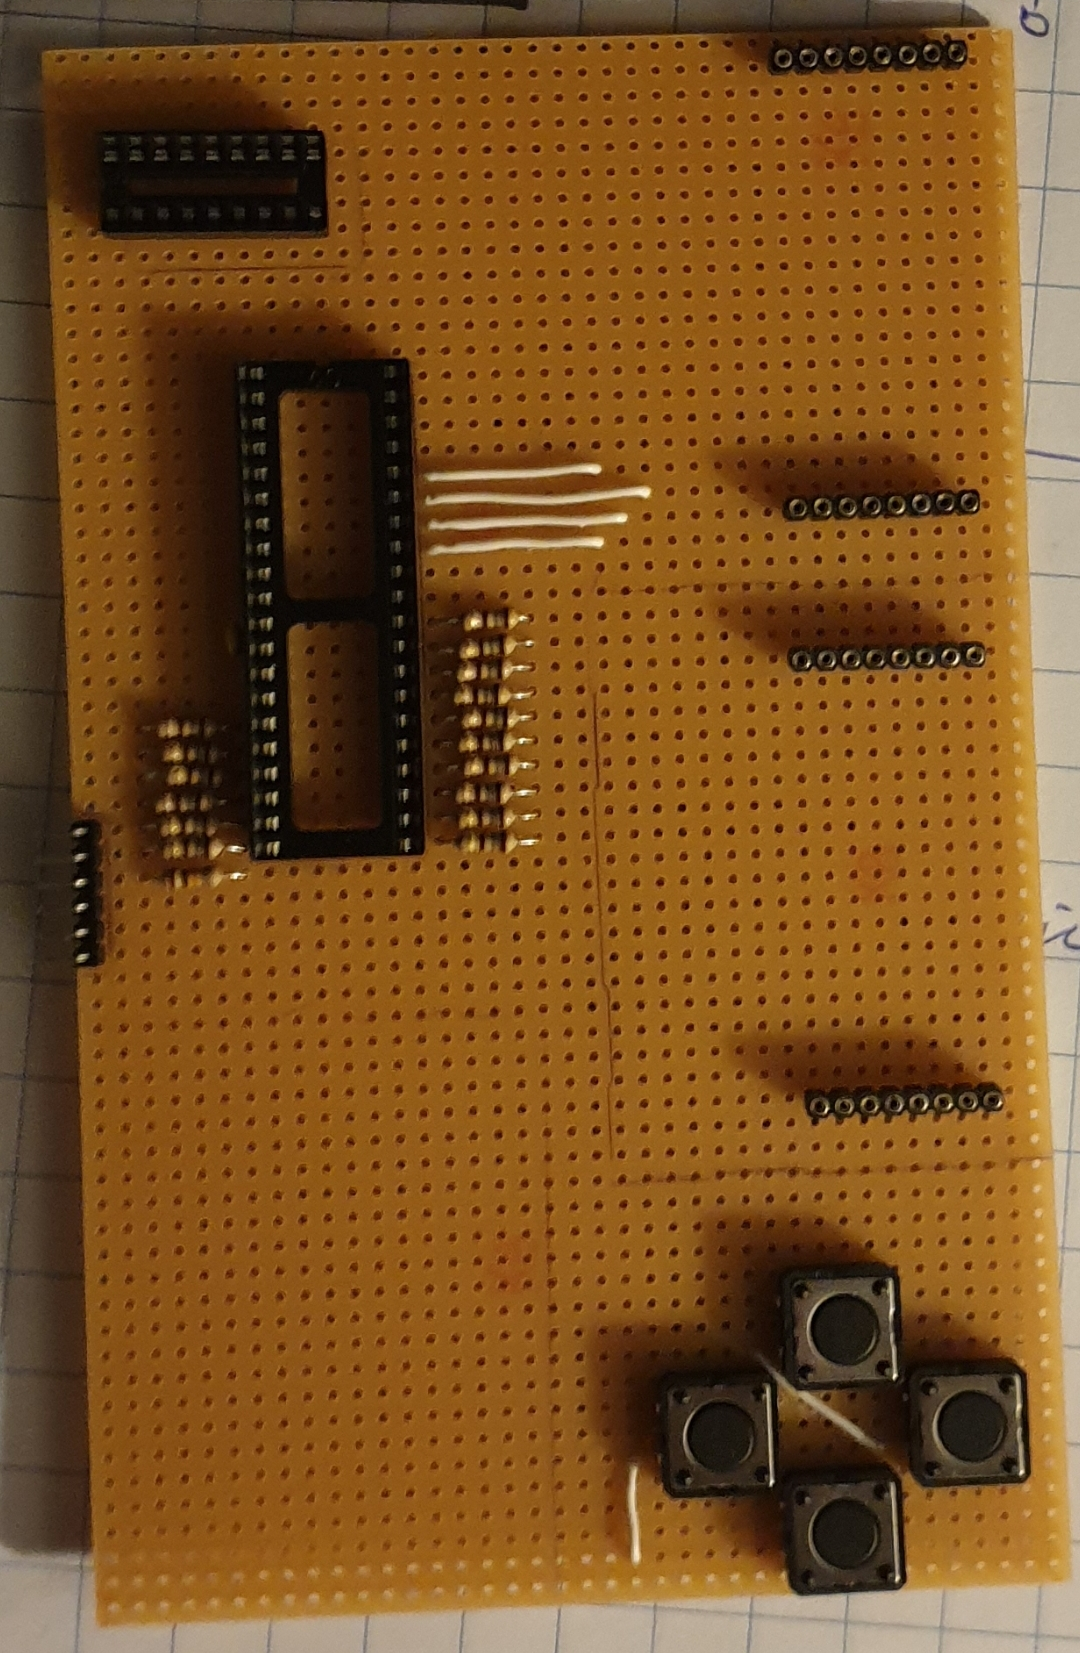
\includegraphics[width=0.612\columnwidth]{voor_voor.jpg}
    \caption{Foto van de voorkant van de Tetris gameboy, vóór de (meeste) bedradingen.}
    \label{fig:voorvoor}
\end{figure}
\begin{figure}[h]
    \centering
    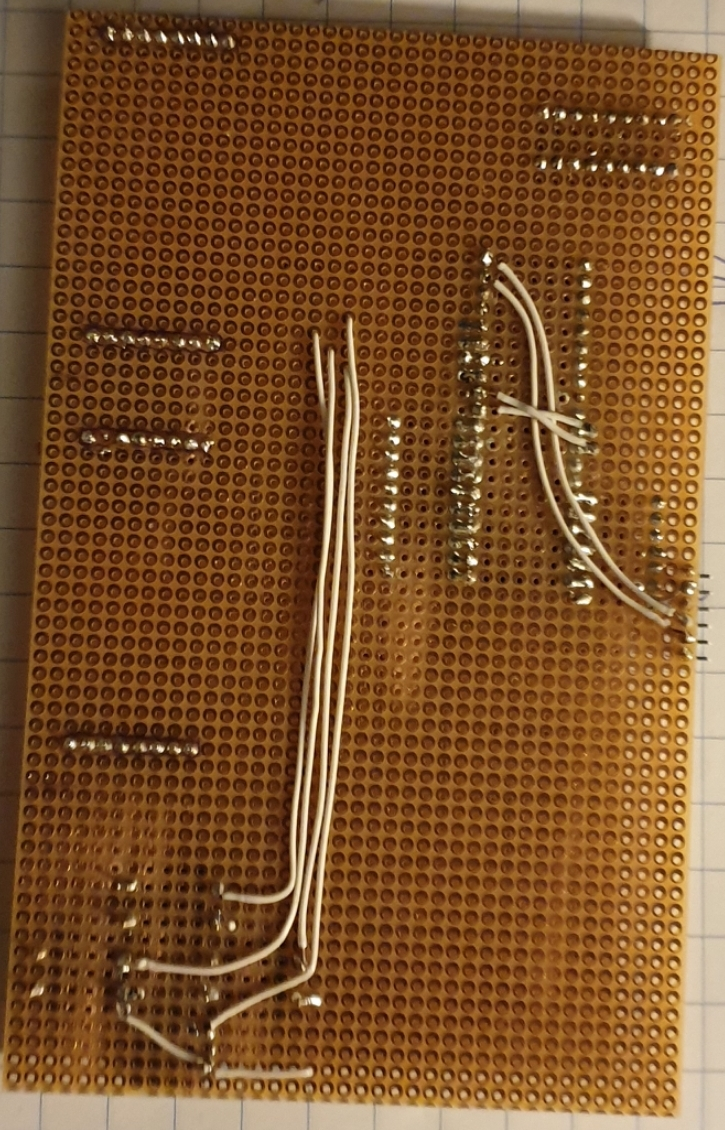
\includegraphics[width=0.612\columnwidth]{voor_achter.jpg}
    \caption{Foto van de achterkant van de Tetris gameboy, vóór de (meeste) bedradingen.}
    \label{fig:voorachter}
\end{figure}
\pagebreak
\\
Zie figuur \ref{fig:navoor} en \ref{fig:naachter} van de vóór- en achterkant van de Tetris gameboy, van ná de bedradingen.
\begin{figure}[h]
    \centering
    \includegraphics[width=0.6\columnwidth]{na_voor.jpg}
    \caption{Foto van de voorkant van de Tetris gameboy, ná de bedradingen.}
    \label{fig:navoor}
\end{figure}
\begin{figure}[h]
    \centering
    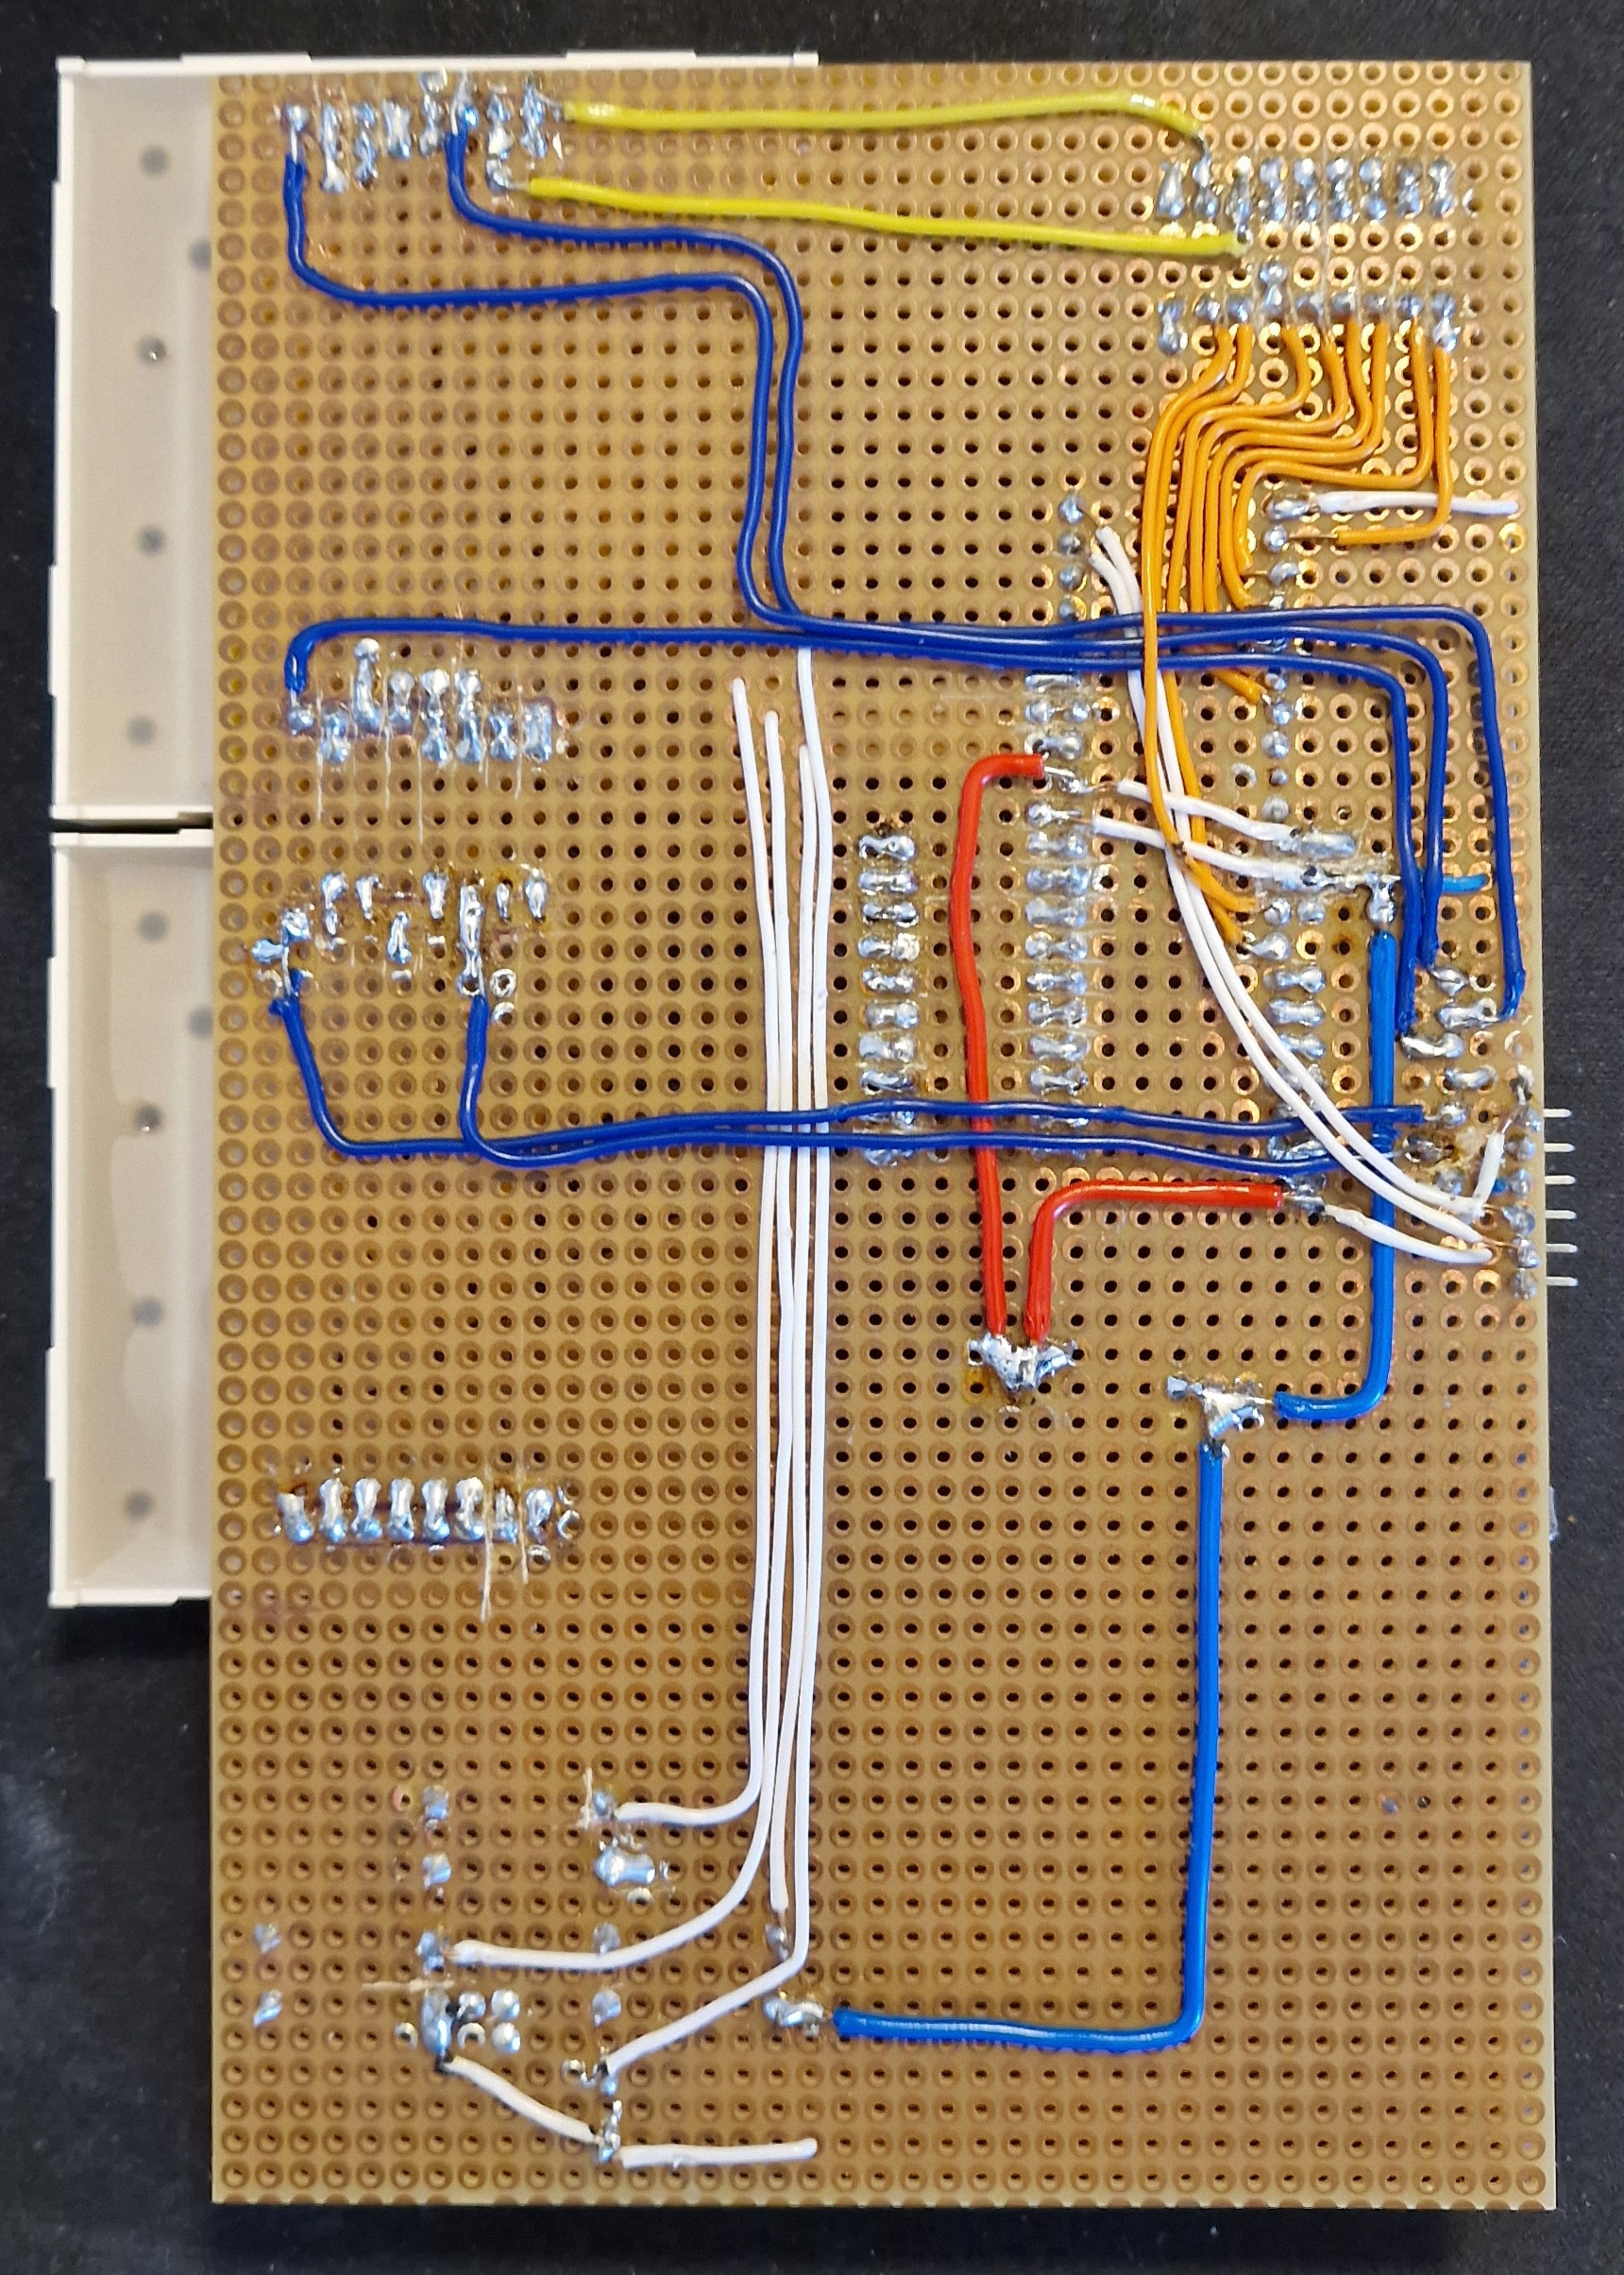
\includegraphics[width=0.6\columnwidth]{na_achter.jpg}
    \caption{Foto van de achterkant van de Tetris gameboy, ná de bedradingen.}
    \label{fig:naachter}
\end{figure}\\
In figuur \ref{fig:naachter} is te zien dat bij de bovenste socket van onderste matrix dat de soldering niet netjes is gedaan. 
Dit komt, omdat een aantal pinnen van de eerst gesoldeerde socket intern kapot waren (tulpcontact was defect). Daarom moest de hele socket gedemonteerd en vervangen worden met behulp van een desoldeerpomp. 
Daarna moest er een nieuwe socket in gesoldeerd worden, maar omdat de desoldeerpomp de meeste koperen eilandjes eruit had gezogen, hechtte het soldeertin niet meer goed aan de perfboard, waardoor het soldeertin direct aan verbindingsdraadje gehecht moest worden. Daarom zien de soldeerresultaten bij die socket er minder goed uit in vergelijking met de rest. 
Het verschil tussen vóór en ná de soldering van die socket is terug zien in figuur \ref{fig:voorachter} en in figuur \ref{fig:naachter}. Voor de rest is het resultaat best netjes en was het solderen redelijk goed te doen. 
\subsection{Tetris Gameboy}
\label{subsec:results:tetrisgame}
Onder dit kopje worden er foto's laten zien van dat de Tetris gameboy succesvol werkt. In figuur \ref{fig:Tstart} is er een foto te zien waarbij op de LED matrixen te zien zijn dat het Tetris spel foutloos opstart. 
In figuur \ref{fig:Tpot1} en \ref{fig:Tpot2} is de Tetris gameplay te zien, hierbij is de eerste foto eerder in het potje gemaakt, en de tweede foto is later in het potje gemaakt. 
Tenslotte in figuur \ref{fig:TpotScore} is te zien dat het potje is afgelopen en dat de score wordt weer gegeven (score: 3).
\begin{figure}[h]
    \centering
    \includegraphics[width=0.6\columnwidth]{Tstart.jpg}
    \caption{Foto van de start-up van het Tetris spel.}
    \label{fig:Tstart}
\end{figure}
\begin{figure}[h]
    \centering
    \includegraphics[width=0.6\columnwidth]{Tpot1.jpg}
    \caption{De eerste foto die hoort bij het potje Tetris.}
    \label{fig:Tpot1}
\end{figure}
\pagebreak
\begin{figure}[h]
    \centering
    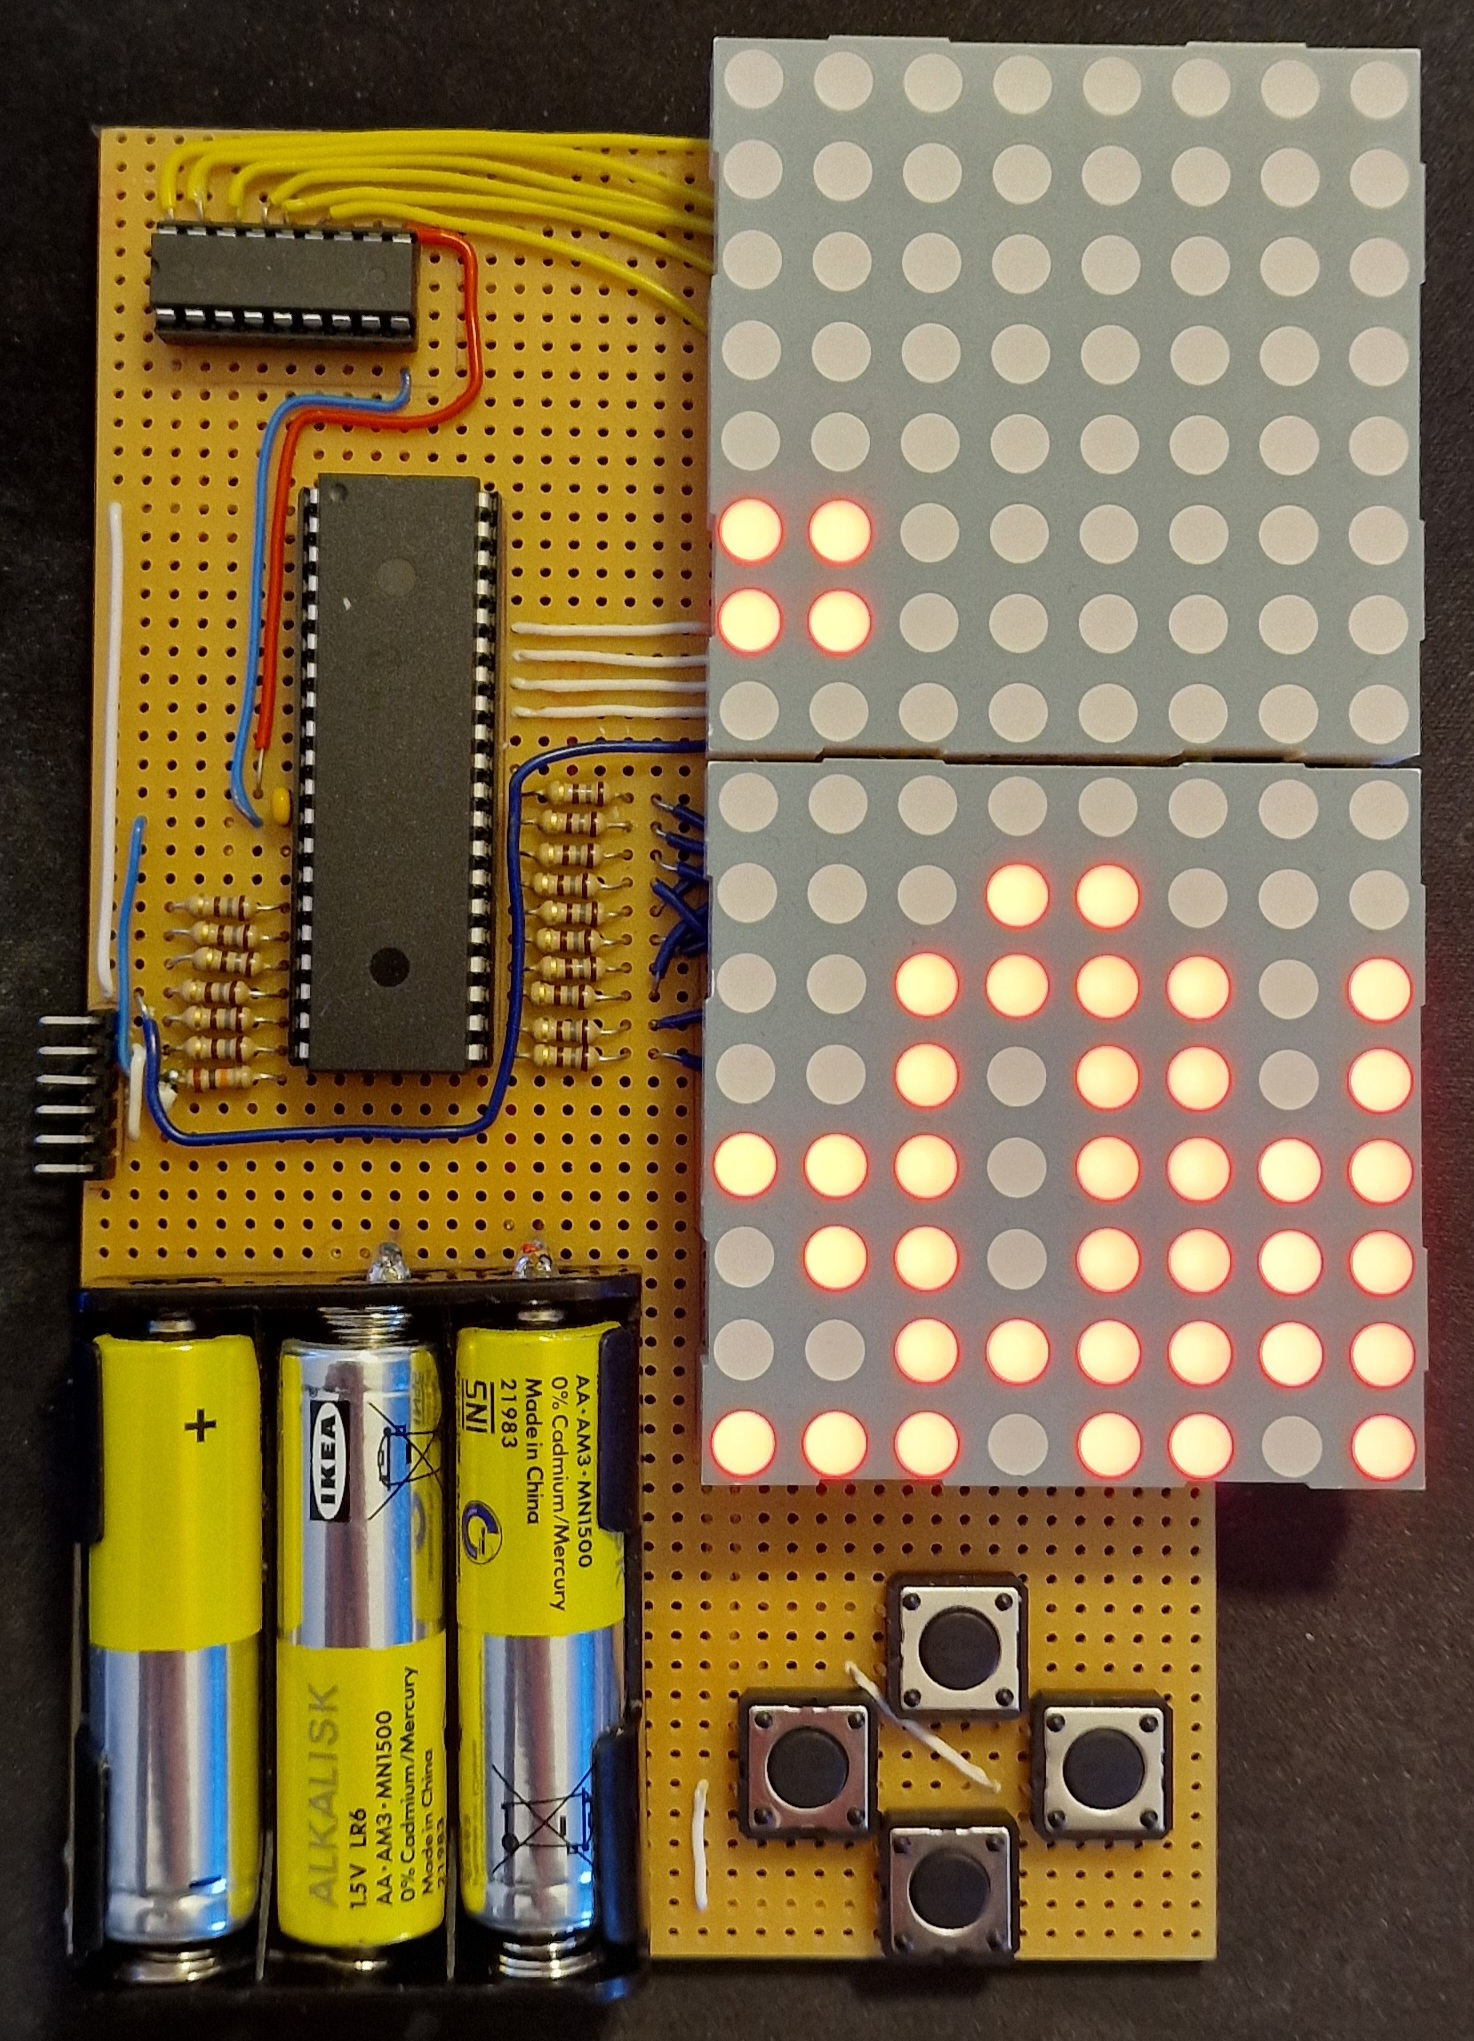
\includegraphics[width=0.6\columnwidth]{Tpot2.jpg}
    \caption{De tweede foto die hoort bij het potje Tetris.}
    \label{fig:Tpot2}
\end{figure}
\begin{figure}[h]
    \centering
    \includegraphics[width=0.6\columnwidth]{TpotScore.jpg}
    \caption{Foto van dat de score te zien is, omdat het game-over is.}
    \label{fig:TpotScore}
\end{figure}\\
De resultaten zijn prima, aangezien alles werkt. De batterijhouder is bijvoorbeeld links onder is geplaatst, omdat daar een betere grip zit voor de linker hand. 
De knopjes zitten dan uiteraard rechts georiënteerd van de batterijhouder.

Hieronder nog even samengevat wat de knopjes deden:\\
De bovenste knop zorgt ervoor dat de Tetromino's draaibaar zijn. De onderste knop zorgt ervoor dat de Tetromino's versneld naar beneden vallen. 
De rechter knop zorgt ervoor dat de Tetromino's naar rechts verplaatst kunnen worden. De linker knop zorgt ervoor dat de Tetromino's naar links verplaatst kunnen worden. 
\pagebreak